\section{Introduction}
\subsection{}
\begin{frame}
  \frametitle{Motivation}
  \begin{itemize}
    \item Era of cloud computing
%     \item Computational resources on demand
    \item Trend goes to Everything as a Service
    \item Still missing: Optimization as a Service
  \end{itemize}
\end{frame}

\begin{frame}
  \frametitle{Optimization}
  \begin{itemize}
    \item Task of finding minimum/maximum of an objective function
%     \item Used in many different areas (robotics, navigation, ...)
    \item No exact solving mechanism available for most real-world problems $\rightarrow$ improve solution iteratively
  \end{itemize}
  \vspace{.5em}
  \begin{center}
    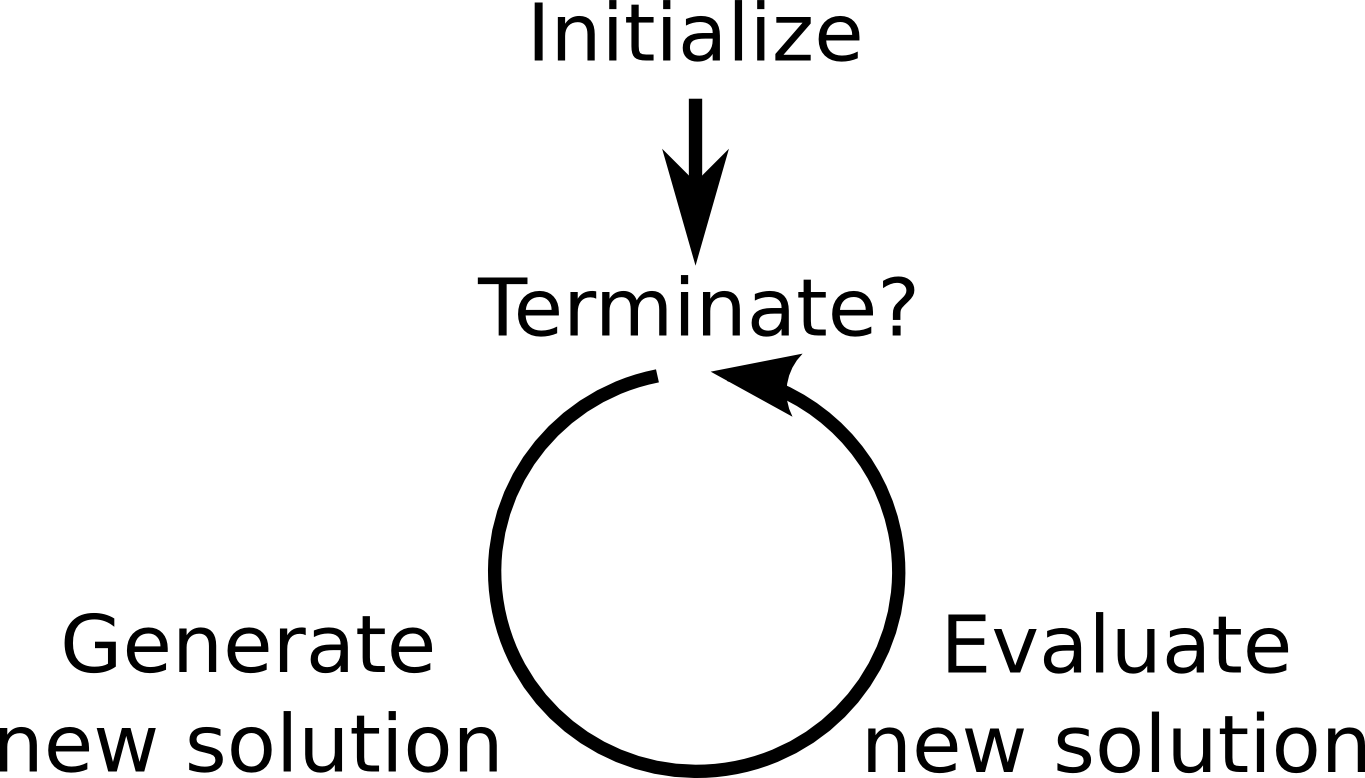
\includegraphics[width=40mm]{iterative.png}
  \end{center}
\end{frame}

\begin{frame}
  \frametitle{Bio-inspired Optimization Techniques}
  \begin{itemize}
    \item Approximation technique: trade accuracy for speed
%     \item Subfamily of metaheuristics
    \item Mimic behaviours observed in nature: Genetic Algorithm (GA), Particle Swarm Optimization (PSO), Ant Colony Optimization (ACO), ...
    \item Main difference between algorithms: solution generation
  \end{itemize}
  \begin{center}
    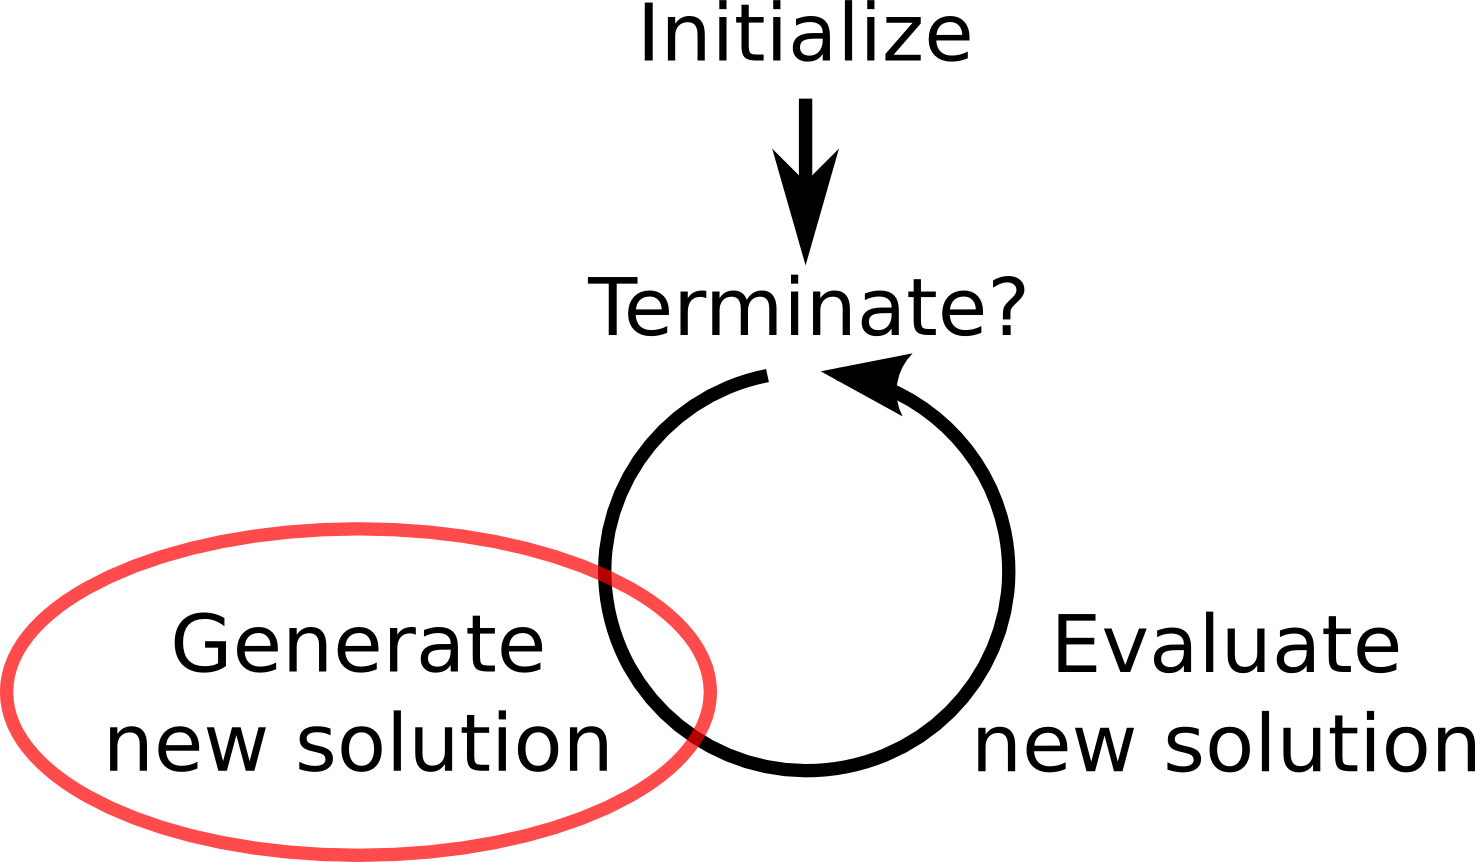
\includegraphics[width=40mm]{bioopt-difference.png}
  \end{center}
\end{frame}

% \begin{frame}
%   \frametitle{(Bio-inspired) Optimization as a Service}
%   \begin{itemize}
%     \item Provide easy access to optimization techniques for large audience
%     \item Leverage cloud capabilities:
%     \begin{itemize}
%       \item (Unlimited) resources on demand
%       \item Don't care about hardware, software, maintenance, ...
%       \item Parallel algorithm execution to increase speed / solve bigger problems
%       \item Simple access
%     \end{itemize}
%   \end{itemize}
%   \vspace{1em}
%   Implementation and execution of algorithms in the cloud differs between providers
% \end{frame}

\begin{frame}
  \frametitle{Apache Hadoop}
  \begin{itemize}
    \item Hadoop is basis layer for implemented framework
    \item ``OS'' for distributed systems
    \item Suited for cloud usage, runs also on single machine e.g. for development
    \item Widely deployed and used system (easy to find / switch provider)
%     \item Known for MapReduce
  \end{itemize}
%   \vspace{1em}
%   $\rightarrow$ use Hadoop as abstraction over different cloud providers
\end{frame}

\begin{frame}
  \frametitle{MapReduce?}
  \begin{itemize}
    \item MapReduce great for problems that can be structured into map and reduce tasks
    \item Not so good for iterative problems:
    \begin{itemize}
      \item Data forwarding through file system (slow)
      \item Check for termination criteria is outside of scope
      \item Computation must be decomposable into map and reduce steps
%       \item Old MapReduce (before 2014): Fixed number of map and reduce slots in cluster, poor resource usage likely
    \end{itemize}
  \end{itemize}
  \begin{center}
    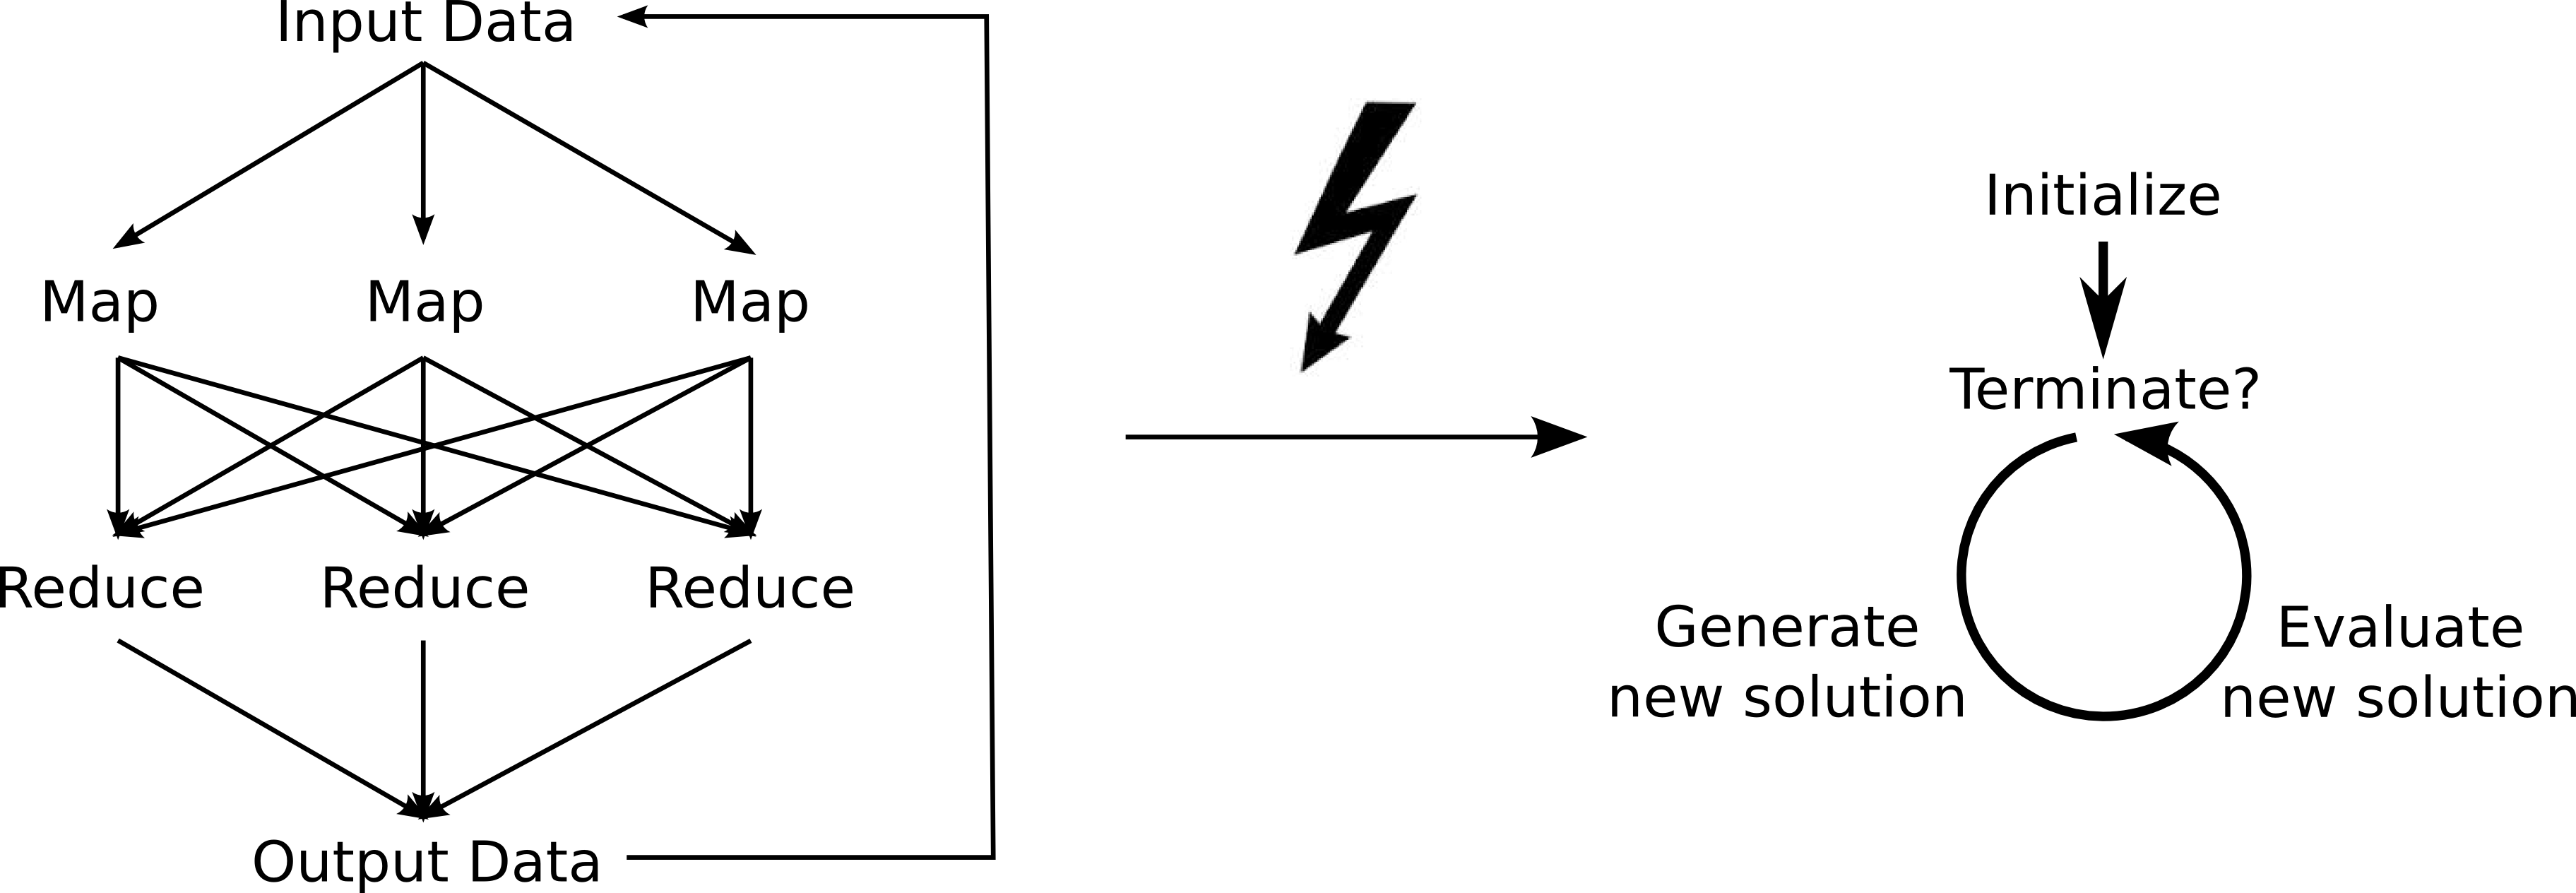
\includegraphics[width=80mm]{mapreduce-to-iterative.png}
  \end{center}
\end{frame}

\begin{frame}
  \frametitle{Better solution}
  In 2014, Hadoop introduced YARN (Yet Another Resource Manager):
  \begin{itemize}
    \item Flexible usage of resources
    \item Enables arbitrary computation models
    \item Gains attraction from developers and cloud providers
  \end{itemize}
  \vspace{1em}
  Low level, verbose and complex API
%   Still low level, verbose and complex API
\end{frame}

\begin{frame}
  \frametitle{Requirements for Optimization as a Service}
  \begin{itemize}
    \item Basis layer over cloud $\rightarrow$ Hadoop + YARN
    \item Need simple framework for implementation and execution of (bio-inspired) optimization techniques $\rightarrow$ \textbf{Biohadoop}
    \begin{itemize}
      \item Based on Hadoop + YARN
      \item Simple API with support for parallelization
    \end{itemize}
    \item Interface to interact with Service (not part of this thesis)
  \end{itemize}
  \begin{center}
    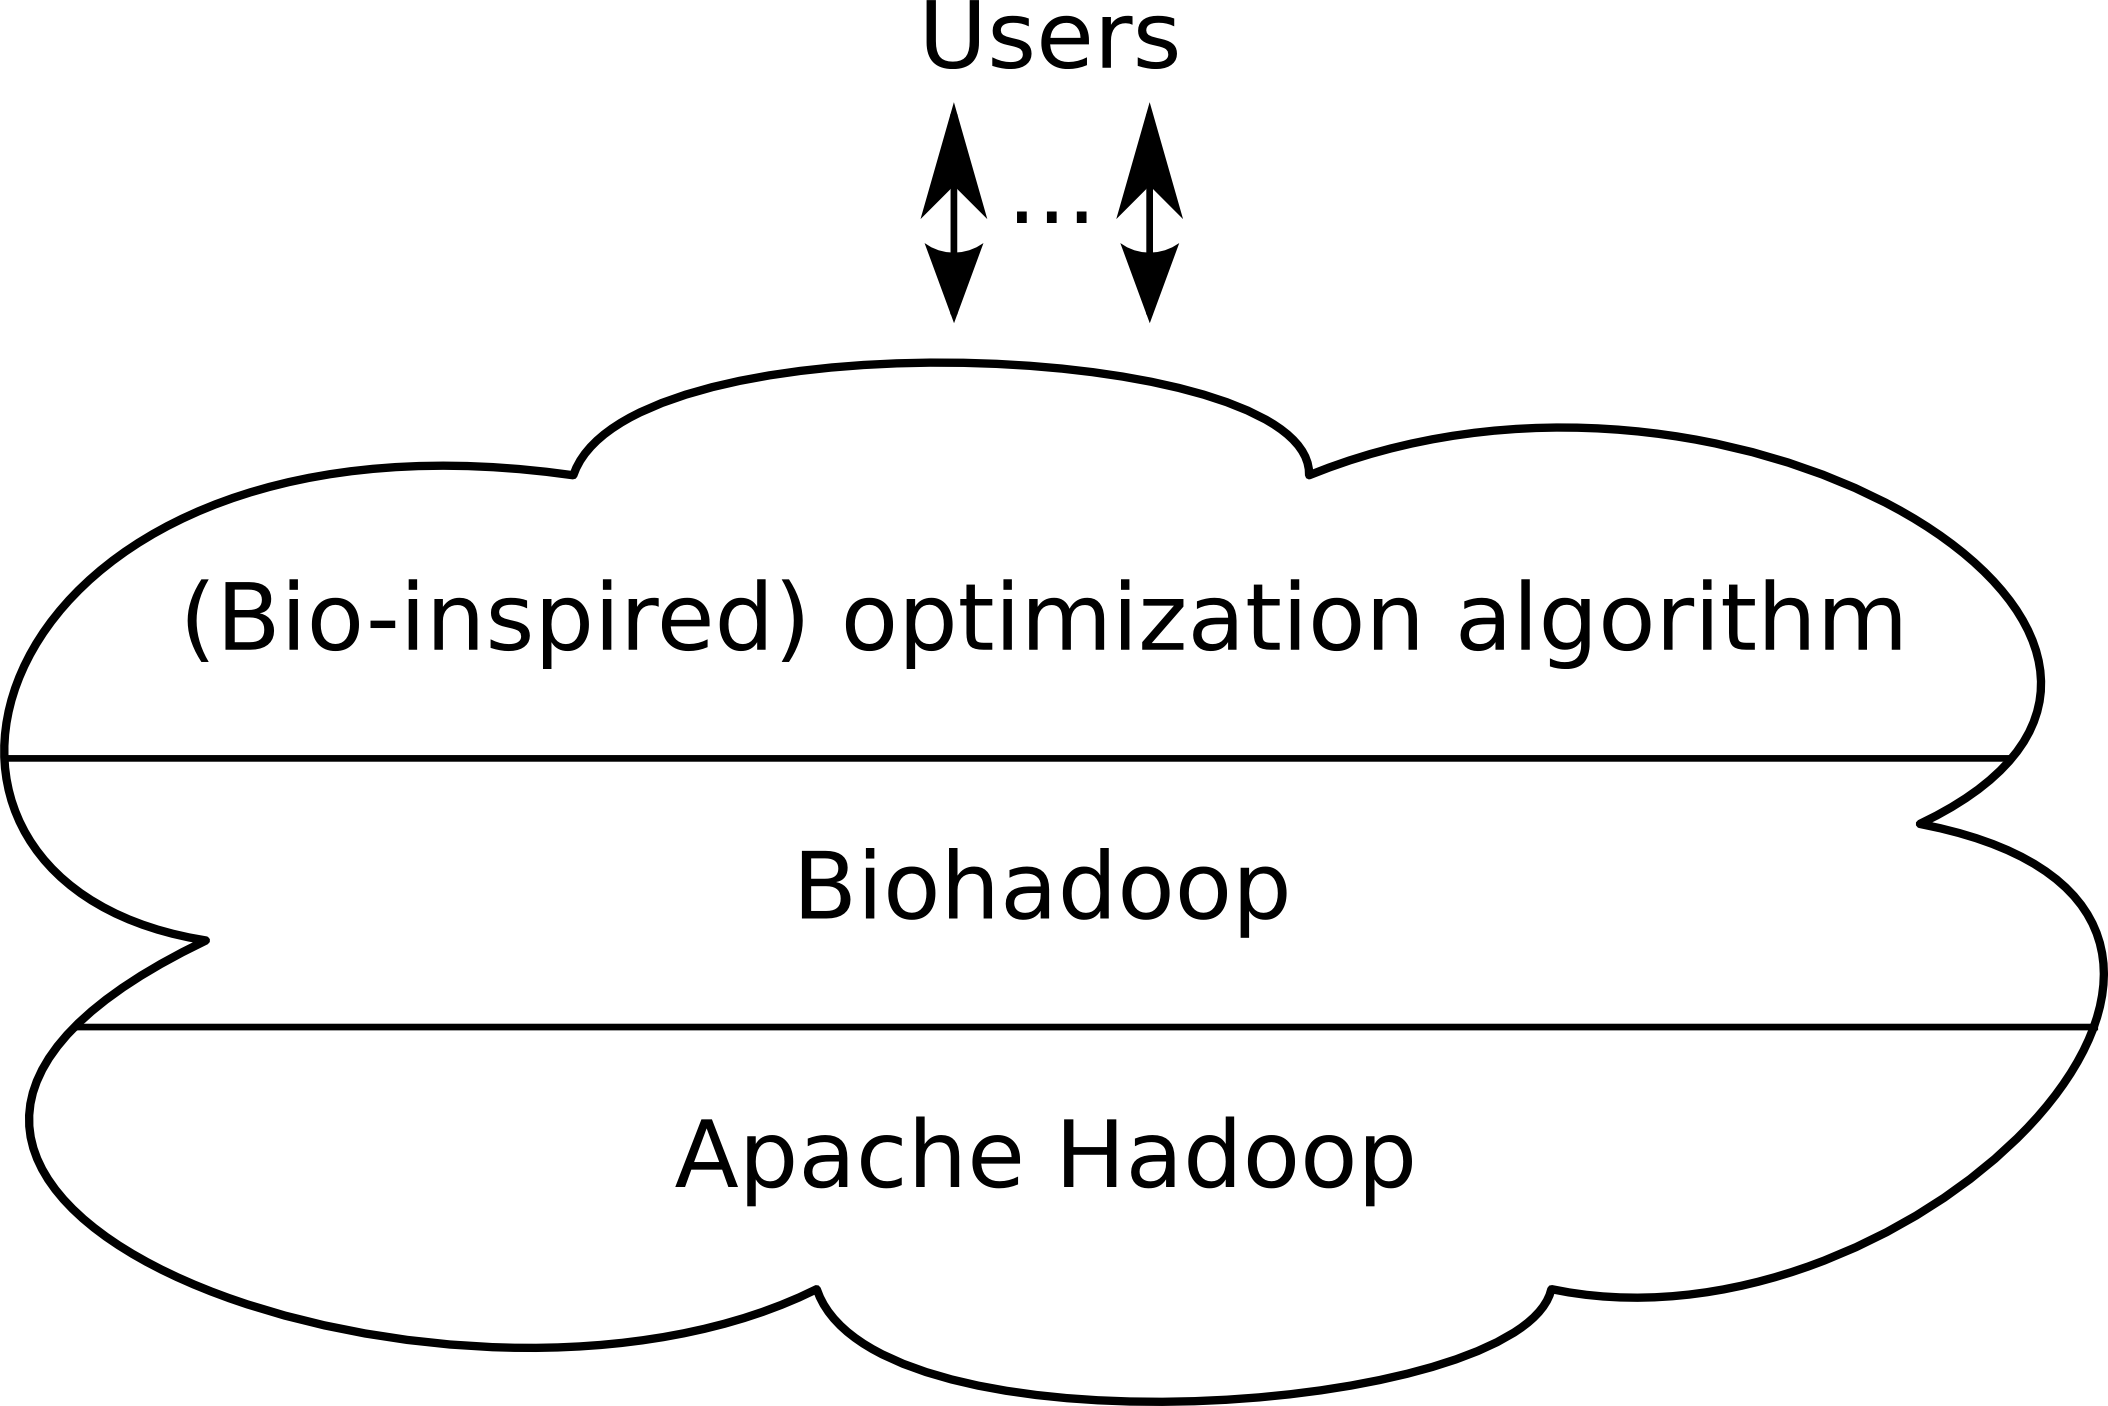
\includegraphics[width=60mm]{opt-as-a-service.png}
  \end{center}
\end{frame}